\documentclass{beamer}
\usepackage{amsmath}
\usepackage{hyperref}
\usepackage{listings}
\usepackage{xcolor}
\hypersetup{colorlinks=true, citecolor=blue, filecolor=blue, linkcolor=blue, urlcolor=blue}
\definecolor{codegreen}{rgb}{0,0.6,0}
\definecolor{codegray}{rgb}{0.5,0.5,0.5}
\definecolor{codepurple}{rgb}{0.58,0,0.82}
\definecolor{backcolour}{rgb}{0.95,0.95,0.92}
 
\lstdefinestyle{mystyle}{
    backgroundcolor=\color{backcolour},   
    commentstyle=\color{codegreen},
    keywordstyle=\color{magenta},
    numberstyle=\tiny\color{codegray},
    stringstyle=\color{codepurple},
    basicstyle=\ttfamily\footnotesize,
    breakatwhitespace=false,         
    breaklines=true,                 
    captionpos=b,                    
    keepspaces=true,                 
    %numbers=left,                    
    numbersep=5pt,                  
    showspaces=false,                
    showstringspaces=false,
    showtabs=false,                  
    tabsize=2
}
 
\lstset{style=mystyle}

\mode<presentation> {

% The Beamer class comes with a number of default slide themes
% which change the colors and layouts of slides. Below this is a list
% of all the themes, uncomment each in turn to see what they look like.

%\usetheme{default}
\usetheme{AnnArbor}
%\usetheme{Antibes}
%\usetheme{Bergen}
%\usetheme{Berkeley}
%\usetheme{Berlin}
%\usetheme{Boadilla}
%\usetheme{CambridgeUS}
%\usetheme{Copenhagen}
%\usetheme{Darmstadt}
%\usetheme{Dresden}
%\usetheme{Frankfurt}
%\usetheme{Goettingen}
%\usetheme{Hannover}
%\usetheme{Ilmenau}
%\usetheme{JuanLesPins}
%\usetheme{Luebeck}
%\usetheme{Madrid}
%\usetheme{Malmoe}
%\usetheme{Marburg}
%\usetheme{Montpellier}
%\usetheme{PaloAlto}
%\usetheme{Pittsburgh}
%\usetheme{Rochester}
%\usetheme{Singapore}
%\usetheme{Szeged}
%\usetheme{Warsaw}

% As well as themes, the Beamer class has a number of color themes
% for any slide theme. Uncomment each of these in turn to see how it
% changes the colors of your current slide theme.

%\usecolortheme{albatross}
%\usecolortheme{beaver}
%\usecolortheme{beetle}
%\usecolortheme{crane}
%\usecolortheme{dolphin}
%\usecolortheme{dove}
%\usecolortheme{fly}
%\usecolortheme{lily}
%\usecolortheme{orchid}
%\usecolortheme{rose}
%\usecolortheme{seagull}
%\usecolortheme{seahorse}
%\usecolortheme{whale}
%\usecolortheme{wolverine}

%\setbeamertemplate{footline} % To remove the footer line in all slides uncomment this line
\setbeamertemplate{footline}[page number] % To replace the footer line in all slides with a simple slide count uncomment this line

\setbeamertemplate{navigation symbols}{} % To remove the navigation symbols from the bottom of all slides uncomment this line
}

\usepackage{graphicx} % Allows including images
\usepackage{booktabs} % Allows the use of \toprule, \midrule and \bottomrule in tables
%\usepackage {tikz}
\usepackage{tkz-graph}
\GraphInit[vstyle = Shade]
\tikzset{
  LabelStyle/.style = { rectangle, rounded corners, draw,
                        minimum width = 2em, fill = yellow!50,
                        text = red, font = \bfseries },
  VertexStyle/.append style = { inner sep=5pt,
                                font = \normalsize\bfseries},
  EdgeStyle/.append style = {->, bend left} }
\usetikzlibrary {positioning}
%\usepackage {xcolor}
\definecolor {processblue}{cmyk}{0.96,0,0,0}
%----------------------------------------------------------------------------------------
%	TITLE PAGE
%----------------------------------------------------------------------------------------

\title[Surrogate models]{Numerical Optimization 14: Surrogate models} %

\author{Qiang Zhu} % Your name
\institute[University of Nevada Las Vegas] % Your institution as it will appear on the bottom of every slide, may be shorthand to save space
{
University of Nevada Las Vegas\\ % Your institution for the title page
\medskip
}
\date{\today} % Date, can be changed to a custom date

\begin{document}

\begin{frame}
\titlepage % Print the title page as the first slide
\end{frame}

\begin{frame}
\frametitle{Overview} % Table of contents slide, comment this block out to remove it
\tableofcontents % Throughout your presentation, if you choose to use \section{} and \subsection{} commands, these will automatically be printed on this slide as an overview of your presentation
\end{frame}

%----------------------------------------------------------------------------------------
%	PRESENTATION SLIDES
%----------------------------------------------------------------------------------------

%------------------------------------------------

\section{Surrogate Models}
\begin{frame}{Surrogate Models}
The \textcolor{blue}{surrogate models} are designed to be smooth and inexpensive to evaluate so that they can be efficiently optimized from the given sampling points. A surrogate model $\hat{f}$ parameterized by $\theta$ is designed to mimic the true objective function $f$. The parameters $\theta$ can be adjusted to fit the model based on samples collected from $f$. 

Suppose we have 
\begin{itemize}
    \item $m$ design points: $\{x^1, x^2, \cdots, x^m\}$
    \item associated function evaluations: $\{y^1, y^2, \cdots, y^m\}$
\end{itemize}
For a particular set of parameters, the model will predict
\begin{equation*}
    \hat{y} = \{\hat{f}_\theta(x^1), \hat{f}_\theta(x^2), \cdots, \hat{f}_\theta(x^m)\}
\end{equation*}

In turn, this is a minimization problem
\begin{equation*}
    \underset{\theta}{\min} = ||y-\hat{y}||
\end{equation*}
\end{frame}

\section{Linear Models}
\begin{frame}{Linear Models}
A simple surrogate model is the linear model, which has the form

\begin{gather*}
    \hat{f} = w_0 + \boldsymbol{w}^T x ~~~~~~~~~~~~ \theta= \{w_0, \boldsymbol{w}\}
\end{gather*}
For an $n$-dimensional design space, the linear model has $n+1$ parameters, and thus requires at least $n+1$ samples to fit unambiguously.

Instead of having both $w$ and $w_0$ as parameters, it is common to construct a single vector of parameters $\theta = [w_0, \boldsymbol{w}]$ and prepend 1 to the vector x to get
\begin{equation*}
    \hat{f} = \boldsymbol{\theta}^T \boldsymbol{x}
\end{equation*}

Finding an optimal $\boldsymbol{\theta}$ requires solving a linear regression problem:
\begin{equation*}
    \underset{\theta}{\min}~||\boldsymbol{y}-\hat{\boldsymbol{y}}|| ~~\textrm{or}~~ ||y-\boldsymbol{X\theta}||
\end{equation*}
where $\boldsymbol{X}$ is a design matrix, $[(\boldsymbol{x}^1)^T; \cdots; (\boldsymbol{x}^m)^T]$

\end{frame}

\section{Basis Functions}
\begin{frame}{Basis Functions}
The linear model is a linear combination of the components of $\boldsymbol{x}$:
\begin{equation*}
    \hat{f}(\boldsymbol{x}) = \theta_1 x_1 + \cdots + \theta_n x_n = \sum_{i=1}^n \theta_i x_i = \boldsymbol{\theta}^T \boldsymbol{x}
\end{equation*}
which is a specific example of a more general linear combination of basis functions.
\begin{equation*}
     \hat{f}(\boldsymbol{x}) = \theta_1 b(x_1) + \cdots + \theta_n b(x_n) = \sum_{i=1}^n \theta_i b(x_i) = \boldsymbol{\theta}^T b(\boldsymbol{x})
\end{equation*}

Linear models cannot capture nonlinear relations. There are a variety of other families of basis functions that can represent more expressive surrogate models. The remainder of this section discusses a few common families.

\end{frame}

\begin{frame}{Polynomial Basis Functions}
Polynomial basis functions consist of a product of design vector components, each raised to a power. Linear basis functions are a special case of polynomial basis functions.

In one dimension, a polynomial model of degree $k$ has the form
\begin{equation*}
    \hat{f}(x) = \theta_0 + \theta_1 x + \theta_2 x^2 + \cdots = \sum_{i=1}^k \theta_i x^i
\end{equation*}

In two dimensions, a polynomial model of degree $k$ has basis functions of the form
\begin{equation*}
    b_{ij}(\boldsymbol{x}) = x_1^j x_2^j ~~{\textrm{for~}} i, j \in \{0, \cdots, k\}, i+j \leq k
\end{equation*}
\end{frame}

\begin{frame}{Sinusoidal Basis Functions}
Any continuous function over a finite domain can be represented using an infinite set of sinusoidal basis functions. A Fourier series can be constructed for any integrable univariate function $f$ on an interval $[a, b]$

\begin{equation*}
    f(x) = \frac{\theta_0}{2} + \sum_{i=1}^\infty \theta_i^{\sin} \sin \bigg(\frac{2\pi ix}{b-a}\bigg)
    \sum_{i=1}^\infty \theta_i^{\cos} \cos \bigg(\frac{2\pi ix}{b-a}\bigg)
\end{equation*}

where
\begin{equation*}
    \begin{split}
        \theta_0 &= \frac{2}{b-a} \int_a^b f(x)dx \\ 
        \theta_i^{\sin}&= \frac{2}{b-a} \int_a^b f(x)\sin \bigg(\frac{2\pi ix}{b-a}\bigg) dx \\ 
        \theta_i^{\cos}&= \frac{2}{b-a} \int_a^b f(x)\cos \bigg(\frac{2\pi ix}{b-a}\bigg) dx 
    \end{split}
\end{equation*}

\end{frame}


\begin{frame}{Radial Basis Functions}
A radial function $\Psi$ is one which depends only on the distance of a point from some center point $c$, such that it can be written $\Psi(x, c) = \Psi(|x − c|)) = \Psi(r)$.

\begin{figure}
\centering
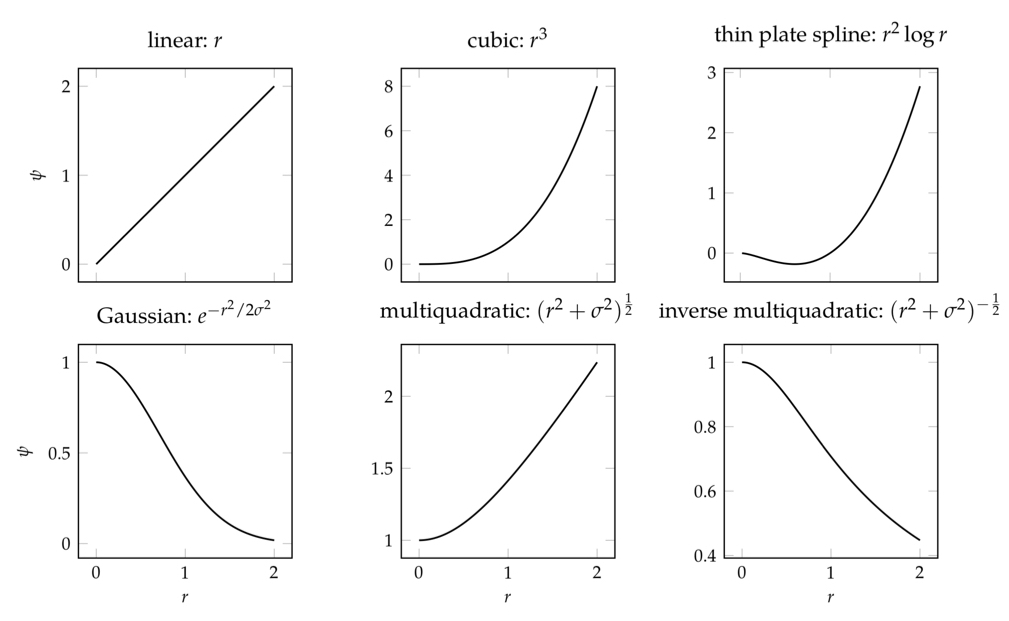
\includegraphics[width=100mm]{Figs/rbf.jpeg}
\end{figure} 

\end{frame}

\section{Fitting Noisy Objective Functions}
\begin{frame}{Fitting Noisy Objective Functions}
Models fit using regression will pass as close as possible to every design point. When the objective function evaluations are noisy, complex models are likely to excessively contort themselves to pass through every point. However, smoother fits are often better predictors of the true underlying objective function. A regularization term is added in addition to the prediction error in order to give preference to solutions with lower weights. The resulting basis regression problem with L2 regularization is:
\begin{equation*}
    \underset{\theta}{\min} ||\boldsymbol{y-B\theta}||^2 + \lambda ||\boldsymbol{\theta}||^2_2
\end{equation*}

The optimal parameter vector is given by:
\begin{equation*}
    \boldsymbol{\theta} = (\boldsymbol{B^TB} + \lambda {\bf I}) \boldsymbol{B^Ty}
\end{equation*}

where \textbf{I} is the identity matrix.
\end{frame}

\section{Model Selection}

\begin{frame}{Model Selection}
So far, we have discussed how to fit a particular model to data. We generally want to minimize generalization error, which is a measure of the error of the model on the full design space, including points that may not be included in the data used to train the model. One way to measure generalization error is to use the expected squared error of its predictions:
\begin{equation*}
    \epsilon_{\textrm{gen}} = \mathbb{E}_{\boldsymbol{x} \sim \boldsymbol{\chi}} \bigg[\bigg(f(x)-\hat{f}(x)\bigg)^2\bigg]
\end{equation*}

which impossible to compute. It may be tempting to estimate the generalization error of a model from the training error by using the mean squared error (MSE) of the model evaluated on the $m$ samples:
\begin{equation*}
    \epsilon_{\textrm{train}} = \frac{1}{m} \sum_i^m \bigg[\bigg(f(x^i)-\hat{f}(x^i)\bigg)^2\bigg]
\end{equation*}

\end{frame}

\begin{frame}{Holdout}
A simple approach to estimating the generalization error is the holdout method, which partitions the available data into a test set $D_h$ with $h$ samples and a training set Dt consisting of all remaining $m-h$ samples. The training set is used to fit model parameters. The held out test set is not used during model fitting, and can thus be used to estimate the generalization error. Different split ratios are used, typically ranging from 50\% train, 50\% test to 90\% train, 10\% test, depending on the size and nature of the dataset. Using too few samples for training can result in poor fits, whereas using too many will result in poor generalization estimates.
\begin{figure}
\centering
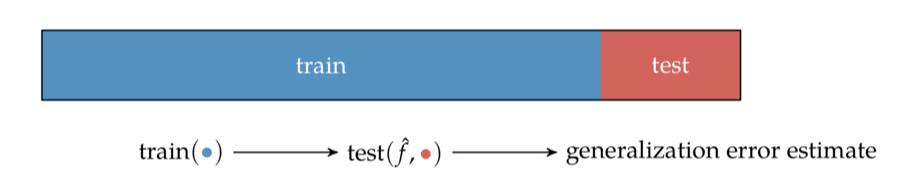
\includegraphics[width=100mm]{Figs/holdout.jpeg}
\end{figure} 

\end{frame}



\begin{frame}{Cross validation}
Here, the original dataset D is randomly partitioned into $k$ sets $D_1, D_2, \cdots, D_k$ of equal, or approximately equal, size. We then train $k$ models, one on each subset of $k-1$ sets, and we use the withheld set to estimate the generalization error. The cross-validation estimate of generalization error is the mean generalization error over all folds   
\begin{figure}
\centering
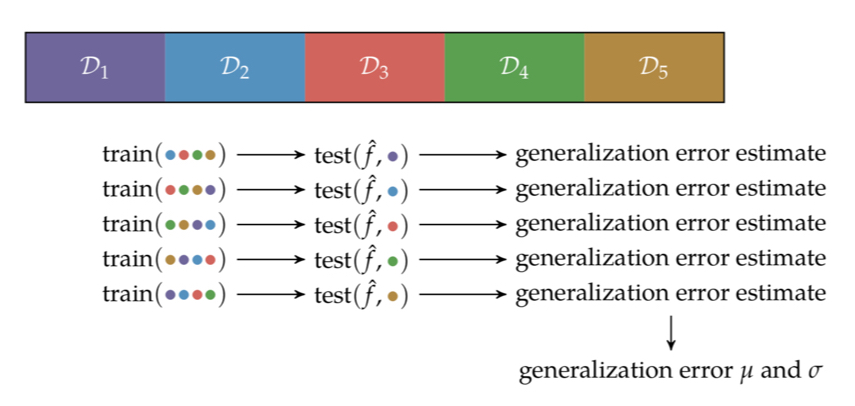
\includegraphics[width=100mm]{Figs/cross-valid.jpeg}
\end{figure} 
\end{frame}

\section{Summary}
\begin{frame}{Summary}
    \begin{itemize}
        \item Surrogate models are function approximations that can be optimized instead of the true, potentially expensive objective function.
        \item Many surrogate models can be represented using a linear combination of basis functions.
        \item Model selection involves a bias-variance trade off between models with low complexity that cannot capture important trends and models with high complexity that overfit to noise.
        \item Generalization error can be estimated using techniques such as hold out,k-fold cross validation, and the bootstrap.
    \end{itemize}
\end{frame}
\end{document}

